\chapter{Implementation} \label{chp:implementation}
This chapter will describe the implementation of the \pub{} and \sub{} as designed in the chapter \ref{chp:design}. In section \ref{sec:verification}, the requirements from the 

\section{Software Components}
\subsection{RTP/RTCP}

\todo{Add in impl. introduction that pub/sub are implemented in perl}

In order for the \pub{} and \sub{} to support sending and receiving RTP and RTCP messages, two C libraries has been compared. As perl has support for wrapping C into shared modules that can be run with a perm module, C has been used.

Two C libraries are compared:

\myparagraph{oRTP} 
The oRTP library is used in \textit{linphone Open-source VoIP}, which is an open-source VoIP solution created and maintained by Belledonne Communications. The oRTP library is released under the GNU GPLv2 and proprietary license meaning the library can be used for open-source projects and in proprietary solutions.
The oRTP library implements RFC3550 with an API that offers a high as well as low level interfacing for sending and receiving RTP and RTCP packets and parsing and composing RTP and RTCP packets. It supports multiple RTP sessions with IPv4 and IPv6 unicast and multicast. Furthermore, it offers support for different profiles, meaning a custom profile can be implrunmodeemented.  oRTP has a sparse documentation with only an autogenerated doxygen, where most of the functionality is described. The source-code comes with simple examples, that explains some of the library's functionality. The library is written in C and can be found in Ubuntu and Debian's packet repository. At the time of writing, the latest commit on their official github has been made 24 days ago which indicates the project is active. In CPAN, an oRTP library can be found, that implements some of the most high level API functions.


\myparagraph{jrtplib}
The jrtplib library is developed at the the Expertise Centre for Digital Media (EDM), a research institute of the Hasselt University. At the time of writing the library has been used in 61 projects listed on \href{http://research.edm.uhasselt.be/jori/cgi-bin/listprojects.py?name=jrtplib}{Project list}. The library is free to use, but must include disclaimer in the source code. The library implements RFC3550 and provides primarily a high level API, that hides most of the implementation details. The library supports parsing, composing, sending and receiving RTP and RTCP messages but does not not implement any profile, The library is written in C++ and well-documented by giving a thoroughly \textit{Getting Started} and includes 7 examples showing how to utilize the functionality of the library. Unfortunately, at the moment of writing the maintainers have not done any commits for the past year.

The libraries are compared based on the following requirements:
\begin{itemize}
	\item \textit{In repository}: From design requirement 4, the library should, if possible, be in the Debian repository.
	\item \textit{RTCP impl.}: The library should implement RTCP, as RTCP is required by the \pub{} and \sub{}.
	\item \textit{Low level API}: As the \pub{} and \sub{} should send RTCP SDEs, RTCP, BYE and RTCP SR.
	\item \textit{Custom RTP Profile}: The library should allow using a custom profile, as the \pub{} and \sub{} requires a custom profile for the non-essential/essential metadata.\todo{Verify requirement}
	\item \textit{API documented}: Preferable to ease implementation of the \pub{} and \sub{}
	\item \textit{Actively Maintained}: Relatively important, in case bugs are discovered.
	\item \textit{IPv6/4 multicast support}: Required by requirement X \todo{Analysis requirement}
	\item \textit{Existing per-binding}: As the \pub{} and \sub{} will be implemented in perl, existing bindings are preferable to ease implementation.
	\item \textit{Multiple RTP session}: Required by design requirement X
	\item \textit{Send \& Receive RTP/RTCP}: is required by \pub{} and \sub{}, respectively.
	\item \textit{Includes examples}: Preferable as it eases implementation.
\end{itemize}

\begin{table}[H]
\centering
\begin{tabular}{@{}|l|l|l@{}|}
\hline
\multicolumn{1}{|l|}{\textbf{Library property}} & \multicolumn{1}{|l|}{\textbf{oRTP}}         & \multicolumn{1}{|l|}{\textbf{jrtplib}}       \\ \midrule
\multicolumn{1}{|l|}{In repository}    & \multicolumn{1}{c|}{\checkmark} & \multicolumn{1}{l|}{} \\ \midrule
\multicolumn{1}{|l|}{RTCP impl.} & \multicolumn{1}{c|}{\checkmark} & \multicolumn{1}{c|}{\checkmark} \\ \midrule
\multicolumn{1}{|l|}{Low level API} & \multicolumn{1}{c|}{\checkmark} & \multicolumn{1}{c|}{} \\ \midrule
\multicolumn{1}{|l|}{Custom RTP Profile} & \multicolumn{1}{c|}{\checkmark} & \multicolumn{1}{c|}{} \\ \midrule
\multicolumn{1}{|l|}{API documented}          & \multicolumn{1}{c|}{\checkmark} & \multicolumn{1}{c|}{\checkmark} \\ \midrule
\multicolumn{1}{|l|}{Actively Maintained}           & \multicolumn{1}{c|}{\checkmark} & \multicolumn{1}{l|}{} \\ \midrule
\multicolumn{1}{|l|}{IPv6 multicast support}           & \multicolumn{1}{c|}{\checkmark} & \multicolumn{1}{c|}{\checkmark} \\ \midrule
\multicolumn{1}{|l|}{IPv4 multicast support}           & \multicolumn{1}{c|}{\checkmark} & \multicolumn{1}{c|}{\checkmark} \\ \midrule
\multicolumn{1}{|l|}{Existing perl-binding}           & \multicolumn{1}{c|}{\checkmark} & \multicolumn{1}{c|}{} \\ \midrule
\multicolumn{1}{|l|}{Multiple RTP sessions support}           & \multicolumn{1}{c|}{\checkmark} & \multicolumn{1}{c|}{\checkmark} \\ \midrule
\multicolumn{1}{|l|}{Send \& Receive}           & \multicolumn{1}{c|}{\checkmark} & \multicolumn{1}{c|}{\checkmark} \\ \midrule
\multicolumn{1}{|l|}{Includes examples}           & \multicolumn{1}{c|}{\checkmark} & \multicolumn{1}{c|}{\checkmark}  \\ \bottomrule
\end{tabular}
\caption{Comparesion of oRTP and jrtplib}
\label{sec:implementation:rtplib}
\end{table}

Based on the number of checkmarks in table \ref{sec:implementation:rtplib}, it has been chosen to use the oRTP library.

\todo{File tree, describe common perl library}
\subsection{Publisher \& Subscriber}

\textit{P1: The \pub{} should be the logical master of the \pro{}}\\
\textit{S1: The \sub{} should be the logical master of the \pro{}}\\

From requirement P1,S2 the \pub{} and \sub{} being the logical masters has been implemented by passing the path to the \con{} and \pro{} to the \sub{} and \pro{} respectively as an argument. This design allows the \pub{} and \sub{} to pass the pipes to the \pro{} and \con{} during run of the \con{} and \pro{}, respectively.

\begin{listing}[H] 
\begin{minted}{python}
./publisher.pl --producer producer.pl
./subscriber.pl --producer consumer.pl
\end{minted}
\caption{Example of publisher.pl run with producer.pl as parameter}
\label{code:critical_section_c}
\end{listing}

This will result in the process tree as depicted in figure \ref{sec:implementation:runmode}.

\begin{listing}[H] 
\begin{minted}{python}
/usr/bin/perl publisher.pl --producer producer.pl
 \_ /usr/bin/perl producer.pl /tmp/pub_data_pipe /tmp/pub_metadata_pipe
 
 /usr/bin/perl subscriber.pl --consumer consumer.pl
 \_ /usr/bin/perl consumer.pl /tmp/pub_data_pipe /tmp/pub_metadata_pipe
\end{minted}
\caption{Example of publisher.pl run as logical master of the producer.pl}
\label{sec:implementation:runmode}
\end{listing}

By running the consumer and producers this way gives modularity in the way the programs can be run, and does not restrict how the \con{} and \pro{} should be implemented.
Three examples are shown, that show how the designed \pros{},\cons{}, \pros{} and \subs{} can be integrated with MCLURS and the streaming idea in section \ref{sec:streamingidea}.

\myparagraph{Grab with static metadata file}
If \program{Grab} is used to deliver data, the programs can be connected as shown in listing \ref{lst:implementation:grab}.

\begin{listing}[H] 
\begin{minted}{bash}
#!/bin/bash
# Named pipes passed as parameters
DATA_PIPE=$1
MD_PIPE=$2

# Provide feedback to the user
echo "Starting producer"

# Set non-essential metadata to Publisher
cat metadata_example.json > $MD_PIPE

# Capture samples and write to datapipe with Fs of 250kHz
/usr/bin/grab -f 2500000 > $DATA_PIPE
\end{minted}
\caption{The listing shows an implementation of a \pro{} that writes metadata and samples to the datapipe and metadatapipe, respectively}
\label{lst:implementation:grab}
\end{listing}

Listing \ref{lst:implementation:grab} shows how the \pro{} could be integrated with \program{grab}.
Metadata is provided by reading the \textit{metadata\_example.json}, and writing it to the metadatapipe.
As \program{grab} does not provide timing of the samples, no RTCP SR messages can be sent.


\myparagraph{Snapshot with dynamic metadata}
In order to use the \pub{} with \program{Snapshot}, the \pro{} must instruct \program{Snapshot} to do repeating snapshots. Furthermore, the \program{Snapshot} must be told where it should write the streams to. This is should in listing \ref{lst:implementation:snapshot1}.
\todo{Describe RTCP SR packet}

\begin{listing}[H] 
\begin{minted}{python}
# Named pipes passed as parameters
DATA_PIPE=$1
MD_PIPE=$2

snapshot = ZMQ(SNAPSHOT)
snapshot.setup()
snapshot.start()
snapshot.snap(start=0,length=4096,count=100,stream=\$1)

\\ Continues
\end{minted}
\caption{The listing shows an implementation of a \pro{} that writes metadata and samples to the datapipe and metadatapipe, respectively}
\label{lst:implementation:snapshot1}
\end{listing}

\todo{Add to design requirements, that RTCP SR must be implemented to provide timestamping.}
From design requirement X, the RTCP SR packets must be sent in order to timestamp the data stream. In order to do this, \program{Snapshot} supports ZMQ clients to query for timing information. When a \textit{Ztatus} command\footnote{Command implemented by the \program{Snapshot} daemon} is received, it sends a reply of the following format:


\begin{listing}[H] 
\begin{minted}{python}
OK Ztatus: WRITER Files 0, Xfr space 49152[ki spl]
READER ACTIVE hix: 0x0000000000824800 [spl]\ 
  tix: 000000000000000000 [spl] now: 0x00002c8008e4ee1e [ns]
\end{minted}
\caption{The listing shows an implementation of a \pro{} that writes metadata and samples to the datapipe and metadatapipe, respectively}
\label{lst:implementation:snapshot1}
\end{listing}


\begin{itemize}
	\item Filter
	\item Grab with metadata from file
	\item Consumer taking data from snapshot and providing dynamic metadata
\end{itemize}


\myparagraph{Inter-Process Communication}
From implementation requirement P2/S2, the non-essential and essential metadata should be passed between the \pub{}/\sub{} and the \con{}/\pro{} using pipes. Three types of pipes are considered:
\begin{itemize}
	\item Named pipe: Named pipes or FIFO pipes in linux usually appear as files, which processes can read from and write to as part of \ac{IPC}. Named pipes are uni-directional, as one process opens the pipe for writing, and another process opens for reading. Having multiple readers from the named pipe is not supported.
	
	\item Unnamed pipe: Unamed pipes are used in linux to chain input/output between processes. As with named pipes, unamed pipes are uni-direction. This is implemented such that standard output(stdout) from one process, is attached to standard in(stdin) to the next process in the chain. As with named pipe, no framing is required.
	
	\item UNIX socket: UNIX sockets work similar to network sockets in linux, but only locally. Many clients can connect to the same server using the UNIX sockets. A UNIX socket appear like a named pipe, as a file. The UNIX socket supports bi-directional communication. 
\end{itemize}

If the \pub{} should use unnamed pipes, an unnamed pipe should be created that attach the unnamed pipe to stdout from the \pro{}, such that data printed from the \pro{} would show up at the other end of the pipe, read by the \pub{}. Another unnamed pipe could be created, that would be attached to standard error(stderr), in order to have two communication channels to pass non-essential/essential metadata and data to the \pub{}. However this design does not allow the \pro{} to generate output, which could be helpful in development, testing and debugging of \cons{}. The same could be applied to the \sub{} and \con{}; however only one communication channel is available from the \sub{} to the \con{}, which is not enough in order to provide essential/non-essential and data to the \con{}.

Unix pipes are not used, as bidirectional communication is not needed. Due to simplicity and using existing linux functionality, the communication between the \pubs{} \subs{} and \con{} and \pro{} is created using named pipes.


\subsection{Publisher}
\subsection{Subscriber}
%\subsection{Runmode}


\section{Metadata}
Metadata must be provided by the \pro{}, as the \pro{} should be implemented to collect essential and non-essential metadata.


\section{Historian}
Due to limited time, a \hist{} has not been implemented. However, two existing alternatives have been compared, in order to verify the architecture works when streams are replayed.

\begin{itemize}
	\item \textit{RTP Tools\footnote{\url{https://www.cs.columbia.edu/irt/software/rtptools/}}} is a suite of RTP programs, used for processing RTP data. The suite consists of rtpdump for saving RTP data, rtpsend for sending RTP packets, rtpplay for replaying recorded RTP data and rtptrans as a translater between unicast and multicast networks.
	
	\item \textit{tcpdump\footnote{\url{https://www.tcpdump.org/tcpdump_man.html}}}. Tcpdump is packet analyser used to monitor network traffic on an interface ;however, it also supports filtering and dumping network traffic into pcap files. These pcap files can then be replayed by programs from the tcpreplay suite.
\end{itemize}

\begin{table}[H]
\centering
\resizebox{\textwidth}{!}{%
\begin{tabular}{|l|c|c|}
\hline
\textbf{}       & \textbf{tcpdump/tcpreplay} & \textbf{rtpdump/rtpplay} \\ \hline
Record duration &                            &                          \\ \hline
IPv6 support    & \checkmark  & X                        \\ \hline
Multiple replay &                            &                          \\ \hline
Replay of RTCP  &          \checkmark                 &         X                 \\ \hline
\end{tabular}%
}
\caption{The table compares tcpdump and RTP tools.}
\label{sec:implementation:tcpreplaytcudmp}
\end{table}


\section{Metadata profile} \label{sec:implemented:metadataprofile} 
A profile must be defined, in order to define a new set of parameters for the RTP packet, in order to use the RTP to carry metadata and events. These parameters are listed below:

\begin{itemize}
	\item \textbf{Packet type}: In the metadata profile, the \textit{Packet type}-field will be used to tell which format the metadata is in. Only two  dataformats are defined, however the RTP profile allows up to $2^7=128$  packet types.
		\begin{itemize}
			\item 0: SDP file. the payload of the RTP packet is in the SDP format.
			\item 1: Non-essential metadata. The payload of the RTP packet is a dump of a perl hashmap. This allows a sender to dump a hashmap of key-value pairs and reconstruct the hashmap on the recipient.
			\item 2: JSON. The payload of the RTP packets are JSON encoded. Each RTP packet contain valid JSON encoded data.
		\end{itemize}
	\item \textbf{Marker bit}: The \textit{Marker}-bit is used to denote whether the RTP packet announces a new frame or provides metadata.
		\begin{itemize}
			\item 0, the RTP packet announces a stream. How the payload is encoded is specified by the \textit{Packet Type}-field.
			\item 1, the RTP packet contains an event. How the content of the packet is encoded is specified by the \textit{Packet Type}-field.
		\end{itemize}
	\item \textbf{32 bit timestamp}
\end{itemize}


\section{Verification} \label{sec:implementation:verification}


\section{Software Components}
The following examples are made in order to show the modularity of the system:



\begin{listing}[h] 
\begin{minted}{python}
	eventHandler = eventLoop()
	
	timerX = Timer(X, callback_Xsec)
	timerY = Timer(Y, callback_Ysec)
	
	eventHandler.add(timerX)
	eventHandler.add(timery)
	
	stream_wellknown    = getStream(fd, callback_wellknown)
	stream_source       = getStream(fd, callback_source)
	stream_sourcepipe   = getStream(source_pipe, callback_sourcepipe)
	stream_metadatapipe = getStream(metadata_pipe, callback_metadatapipe)	
	
	eventHandler.add(stream_wellknown)
	eventHandler.add(stream_source)
	eventHandler.add(stream_sourcepipe)
	eventHandler.add(stream_metadatapipe)
	
	eventHandler.run()
\end{minted}
\caption{Critical section for copying counter value. C version.}
\label{code:critical_section_c}
\end{listing}



\section{Test}
From wireshark after resample:
4096 = payload
8 bytes = data gram
12 bytes rtp header

4116 bytes i total

Compare output of stream with snapshot-file
Write 1XXXE and verify with wireshark dissector
    - in table with output
Two subscribers to one stream - compare data. \# samples, md5 of files.
Record and replay, plot to verify data
Compare RTCP abs. timestamp with expected timestamp form RTP samples.

\section{Timing in RTCP packets}
\begin{align}
	mon_1 &= Monotonic time \\
	realtime &= now \\
	mon_2 &= Monotonic time \\
	offset &= realtime-(mon_1+mon_2)/2 
\end{align}


\section{Ipv6}
   IPv6 sessions are announced on the address FF0X:0:0:0:0:0:2:7FFE
      where X is the 4-bit scope value.  For example, an announcement
      for a link-local session assigned the address
      FF02:0:0:0:0:0:1234:5678, should be advertised on SAP address
      FF02:0:0:0:0:0:2:7FFE.
      

Generation of random IPv6:
Last part of IPv6:
::XXXX = 16 bits
$2^16 = 65536$
 \todo{Compare gstreamer with custom impl.}


\section{Gstreamer}
Gstreaner is a open source tool available, that implements some of the protocols described in section \ref{sec:design:protocols}.
\todo{Describe gstreamer + pros and cons}
Cons:
 - 64bit timestamp injected
 - Does not handle multicast address assignment
Gstreamer is a pipeline based streaming framework that aims to make it easy to work with streams. Gstreamer is plugin based which allows for adding functionality as needed in applications. The idea of plugins is to create plugins are have a well defined responsibility such as reading a file, encoding, playing etc. The plugins are usually connected in gstreamer pipelines, however then can be used in independent applications. Gstreamer plugins are connected using pads, where each plugin can have a source and sink pad. A source pad can then be connected to the next plugin's sink pad. An example of plugins in a pipelines is showed below:
\begin{figure}
	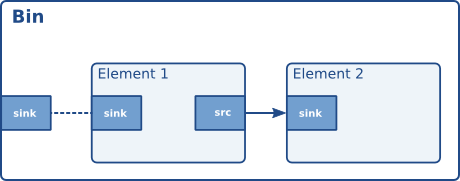
\includegraphics[width=1\textwidth]{figures/bin-element-ghost.png}
\end{figure}

\todo{Describe example figure + rtpbin + rtppay/depay}

\todo{Describe dummy producer.pl}
\section{Only permit one publisher pr. stream}

The test has been conducted by first starting one instance of \program{Publisher} and when it starts to publish data, then a second instance of the \program{Publisher}. Both \program{Publishers} have been given the same highbandwidth IPv6 multicast address, namely FF15::1234.

Listing \ref{lst:implementation:uniquepub1} shows the output from the first \program{Publisher}.

\begin{lstlisting}
Random ip: ff15::1234
Verbose: 5
Executable: producer.pl
"producer.pl" is readable
"producer.pl" is exeutable
Data pipe: /tmp/pipe_publisher_data metadata pipe:/tmp/pipe_publisher_metadata
Waitfor: duration 5.000000 and interval 1.000000
Callback invoked...
Waitfor: wake from sleep at elapsed 1.000000
Callback invoked...
Waitfor: wake from sleep at elapsed 2.000000
Callback invoked...
Waitfor: wake from sleep at elapsed 3.000000
Callback invoked...
Waitfor: wake from sleep at elapsed 4.000000
Callback invoked...
Waitfor: wake from sleep at elapsed 5.000000
Waitfor: loop completed, elapsed 5.000000 of 5.000000
No IPv6 multicast conflict
\end{lstlisting} \label{lst:implementation:uniquepub1}

Listing \ref{lst:implementation:uniquepub2} shows the output from the second instance of the \program{Publisher}.

\begin{lstlisting}
Random ip: ff15::1234
Verbose: 4
Executable: producer.pl
"producer.pl" is readable
"producer.pl" is exeutable
Data pipe: /tmp/pipe_publisher_data metadata pipe:/tmp/pipe_publisher_metadata
Waitfor: duration 5.000000 and interval 1.000000
Callback invoked...
ff15::1234 vs. ff15::1234
Waitfor: loop completed, elapsed 1.000000 of 5.000000
Ipv6 multicast group conflict
New random IPv6 multicast ip: ff15::8a12
Waitfor: duration 5.000000 and interval 1.000000
Callback invoked...
ff15::1234 vs. ff15::8a12
Callback invoked...
ff15::1234 vs. ff15::8a12
Callback invoked...
ff15::1234 vs. ff15::8a12
Callback invoked...
ff15::1234 vs. ff15::8a12
Callback invoked...
ff15::1234 vs. ff15::8a12
Waitfor: loop completed, elapsed 5.000000 of 5.000000
No IPv6 multicast conflict
\end{lstlisting}\label{lst:implementation:uniquepub2}


\section{Verification} \label{sec:design:verification}
Several of the implementation requirements have been addressed in the chapter \ref{sec:implementation}. In order to verify the implementation and there by design works, 7 tests have been conducted.
\todo{Add what has not been fully implemented}

\todo{Describe in list which requirements are tested.}
\begin{itemize}
	\item \textbf{Session Announcement (Essential metadata)}\\
This test aims to verify the Session Announcement Mechanism with Essential metadata works as intended.
	\item \textbf{Presence Mechanism}\\
This test aims to verify the Presence Mechanism works as intended.
	\item IP collision resolver
This test aims to verify the \pub{} is able to generate a new multicast IP if there is a collision.
	\item Subscribe resolve MG
This test verifies the \sub{} can tage a session name, and resolve that into an multicast IP.
	\item Non-essential Metadata
This test verifies non-essential metadata can be sent and received.
	\item Record with tcpdump and replay with tcpreplay and see subscriber get same data.
This test verifies a stream can be recorded and replayed.
	\item Verify RTCP SR timestamps
This test is supposed to verify RTP SR timestamps are working, however at the moment of writing it does not work.
	\item Compare output from \con{} with output from \program{Snapshot}.
This verifies data sent from snapshot is the same as the \con{} receives.
\end{itemize}


\subsection{Session Announcement \& Essential metadata} \label{sec:verify:sessionannouncement}
This test verifies implementation requirement P8,P9 and S3. The goal of the test is to verify a SDP sent by a \pub{}, and verify a \sub{} can join an announced stream. \todo{add essential metdata tot}
The test has been conducted by staring a \pub{} that streams data from a \con{} which interfaces \program{Snapshot}. In order to verify the SDP is sent as an RTP packet, the traffic sent by the \pub{} has been inspected by \program{tcpdump}. Listing \ref{cmd:verify:sdp} shows the SDP packet sent by the \pub{}.

\begin{listing}[H] 
\begin{minted}{bash}
v=0
o=suas 3736400647 3736400647 IN IP4 batbox3
s=My Session
i=A fun session
u=http://www.ecs.soton.ac.uk/fun/
t=3736400647 3736404247
a=tool:publisher.pl uuid: E9A60146-618C
m=audio 5004 RTP/AVP 96
c=IN IP6 ff15::1234/5
a=quality:5
a=rtpmap:96 L16/220500/1
\end{minted}
\caption{SDP printed by the \pub{}}
\label{lst:verify:sdp}
\end{listing}

Figure \ref{lst:verify:tcpdumpsdp} shows the output from \program{tcpdump}.

\begin{listing}[H] 
	\begin{minted}{bash}
sudo tcpdump -i eth0 -X port 5004
11:04:08.895637 IP6 batbox3.local.5004 > ff15::beef.5004: UDP, length 270
        0x0000:  6006 4601 0116 110a fe80 0000 0000 0000  `.F.............
        0x0010:  ba27 ebff fe5e 2624 ff15 0000 0000 0000  .'...^&\$........
        0x0020:  0000 0000 0000 beef 138c 138c 0116 e83d  ...............=
        0x0030:  8000 0000 0001 e240 23e2 c753 763d 300a  .......@#..Sv=0.
        0x0040:  6f3d 7375 6173 2033 3733 3634 3030 3634  o=suas.373640064
        0x0050:  3720 3337 3336 3430 3036 3437 2049 4e20  7.3736400647.IN.
        0x0060:  4950 3420 6261 7462 6f78 330a 733d 4d79  IP4.batbox3.s=My
        0x0070:  2053 6573 7369 6f6e 0a69 3d41 2066 756e  .Session.i=A.fun
        0x0080:  2073 6573 7369 6f6e 0a75 3d68 7474 703a  .session.u=http:
        0x0090:  2f2f 7777 772e 6563 732e 736f 746f 6e2e  //www.ecs.soton.
        0x00a0:  6163 2e75 6b2f 6675 6e2f 0a74 3d33 3733  ac.uk/fun/.t=373
        0x00b0:  3634 3030 3634 3720 3337 3336 3430 3432  6400647.37364042
        0x00c0:  3437 0a61 3d74 6f6f 6c3a 7075 626c 6973  47.a=tool:publis
        0x00d0:  6865 722e 706c 2075 7569 643a 2045 3941  her.pl.uuid:.E9A
        0x00e0:  3630 3134 362d 3631 3843 0a6d 3d61 7564  60146-618C.m=aud
        0x00f0:  696f 2035 3030 3420 5254 502f 4156 5020  io.5004.RTP/AVP.
        0x0100:  3936 0a63 3d49 4e20 4950 3620 6666 3135  96.c=IN.IP6.ff15
        0x0110:  3a3a 3132 3334 2f35 0a61 3d71 7561 6c69  ::1234/5.a=quali
        0x0120:  7479 3a35 0a61 3d72 7470 6d61 703a 3936  ty:5.a=rtpmap:96
        0x0130:  204c 3136 2f32 3230 3530 302f 310a       .L16/220500/1.
	\end{minted}
\caption{The listing shows the output from \program{tcpdump}, listening on the well known multicast group. The bytes shown before the SDP packet is the ethernet header, UDP header and RTP header}
\label{lst:verify:tcpdumpsdp}
\end{listing}

It should be noted that the ASCII encoded content of the payload corresponds to the SDP packet in listing \ref{lst:verify:sdp}. Furthermore, a session is announce in the key starting with \textbf{C=IN...}.

In listing \ref{lst:verify:subsdp} is the output from a \sub{} shown, that receives the SDP.


\begin{listing}[h] 
\begin{minted}{bash}
SDP from 'publisher.pl uuid: E9A60146-618C', format: audio/L16/220500/1,\
	Multicast: ff15::1234:5004
Joining multicast group: ff15::1234:5004
<SDP printet>
Main-loop stopped with retval: NewRtp
Restarting loop due to new RTP stream joined
\end{minted}
\caption{Listing shows the output from a \sub{} that receives the SDP and joins the stream. It should be noted the event-loop is restarted, in order to also listen for the new multicast group}
\label{lst:verify:subsdp}
\end{listing}



\subsection{Presence Mechanism} \label{sec:verify:presencemechanism}
This test verifies implementation requirement P11-13 and S3. The goal of this test is to verify the presence mechanism works in both \sub{} and \pub{}. Due to lack of time, lists maintaining present participants have not been implemented, however RTCP SDES/BYE are sent and received by both \pub{} and \sub{}.
A test was conducted, where the \pub{} is started and some time later the \sub{} is started. The RTCP SDES sent by the \pub{} and \sub{} is shown in figure \ref{fig:verify:wireshark_presence}.

\begin{figure}[H]
	\centering
	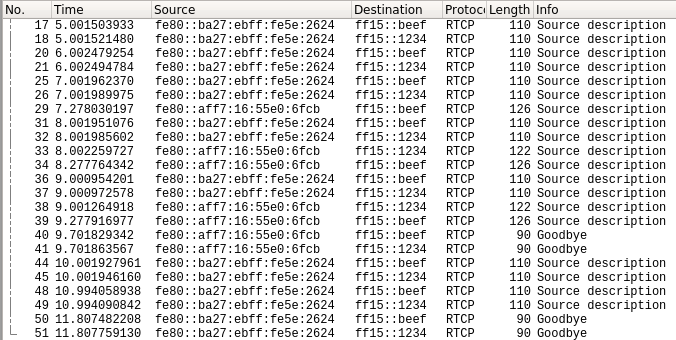
\includegraphics[width=\textwidth]{figures/wireshark_presence}
	\caption{Figure shows output from \program{Wireshark}. It should be noted, that until packet nr.26 is only fe80::ba27:.. sending RTCP SDES, but when \sub{} joins, it starts sending RTCP SDES to both the well known address ff15::beef and the source multicast group ff15::1234.} \label{fig:verify:wireshark_presence}
\end{figure}
From figure \ref{fig:verify:wireshark_presence} the RTCP SDES packets can be seen. Until packet no. 26 is only the \pub{} running. It can be seen that the \pub{} sends its RTCP SDES to both the well known multicast address(ff15::beef) and its source stream (ff15::1234). From packet nr.29, the \sub{} has been started, where it sends out an RTCP SDES to the well known multicast group. It has then joind the source multicast announced by the \pub{} from message no. 32, as the \sub{} sends RTCP SDES to the source stream too. From message no. 40 is the \sub{} gracefully shutting down as it sends a RTCP BYE to both source and well known multicast group. From message no. 50, the \pub{} is gracefully shutting down too.

Listing \ref{lst:verify:rtcpsdes} shows the ouput from a \sub{} receiving and parsing an RTCP SDES packet.

\begin{listing}[h] 
\begin{minted}{bash}
\$VAR1 = bless( {
                 'sdes' => {
                             '6c73c635' => {
                                             'LOC' => '',
                                             'PHONE' => '',
                                             'NAME' => '',
                                             'TOOL' => 'MCLURS',
                                             'NOTE' => '',
                                             'CNAME' => 'suas@batbox3',
                                             'EMAIL' => ''
                                           }
                           }
               }, 'Net::RTCP::Packet' );
\end{minted}
\caption{Listing shows part of the output from a \sub{} receiving and parsing an RTCP SDES packet sent by a \pub{}}
\label{lst:verify:rtcpsdes}
\end{listing}


\subsection{}

\begin{itemize}
	\item Tested with Lua/(post dissector) in wireshark. Transfer chunk of data of 4096 kb(page size) with counter in start of packet. Packet is read from wireshark and by writing dummy producer of 'X' x 4096.

	\item Show Byes are sent when publisher/subscriber are shutdown gracefully

	\item Show essential metadata are sent periodically as json/yml
	\item Show SDES \& BYE to both RTP sessions
	
\end{itemize}


